\documentclass{article}
\usepackage{amsmath, amsthm, amssymb, amsfonts}
\usepackage{thmtools}
\usepackage{graphicx}
\usepackage{setspace}
\usepackage{cancel}
\usepackage{geometry}
\usepackage{float}
\usepackage{hyperref}
\usepackage[utf8]{inputenc}
\usepackage[english]{babel}
\usepackage{framed}
\usepackage[dvipsnames]{xcolor}
\usepackage{tcolorbox}
\usepackage{amsmath}
\usepackage{array}
\usepackage{tikz} 
\usepackage{multirow}
\usepackage{tcolorbox}
\usepackage{xcolor}
\usepackage{tikz-cd}
\usepackage{xcolor}
\usepackage{wasysym}

% Define a new color for the example box



\colorlet{LightGray}{White!90!Periwinkle}
\colorlet{LightOrange}{Orange!15}
\colorlet{LightGreen}{Green!15}

\newcommand{\HRule}[1]{\rule{\linewidth}{#1}}

\colorlet{LightGray}{black!10}
\colorlet{LightOrange}{orange!15}
\colorlet{LightGreen}{green!15}
\colorlet{LightBlue}{blue!15}
\colorlet{LightCyan}{cyan!15}



\declaretheoremstyle[name=Theorem,]{thmsty}
\declaretheorem[style=thmsty,numberwithin=section]{theorem}
\usepackage{tcolorbox} % Add missing package
\tcolorboxenvironment{theorem}{colback=LightGray}

\declaretheoremstyle[name=Definition,]{thmsty}
\declaretheorem[style=thmsty,numberwithin=section]{definition}
\tcolorboxenvironment{definition}{colback=LightBlue}

\declaretheoremstyle[name=Proposition,]{prosty}
\declaretheorem[style=prosty,numberlike=theorem]{proposition}
\tcolorboxenvironment{proposition}{colback=LightOrange}


\declaretheoremstyle[name=Example,]{prosty}
\declaretheorem[style=prosty,numberlike=theorem]{example}
\tcolorboxenvironment{example}{colback=LightOrange}

\declaretheoremstyle[name=Axiom,]{prcpsty}
\declaretheorem[style=prcpsty,numberlike=theorem]{axiom}
\tcolorboxenvironment{axiom}{colback=LightGreen}

\declaretheoremstyle[name=Lemma,]{prcpsty}
\declaretheorem[style=prcpsty,numberlike=theorem]{lemma}
\tcolorboxenvironment{lemma}{colback=LightCyan}





\setstretch{1.2}
\geometry{
    textheight=9in,
    textwidth=5.5in,
    top=1in,
    headheight=12pt,
    headsep=25pt,
    footskip=30pt
}

% ------------------------------------------------------------------------------

\begin{document}

% ------------------------------------------------------------------------------
% Cover Page and ToC
% ------------------------------------------------------------------------------

\title{ \normalsize \textsc{}
		\\ [2.0cm]
		\HRule{1.5pt} \\
		\LARGE \textbf{\uppercase{Lecture 7}}
		\HRule{2.0pt} \\ [0.6cm] \LARGE{}
		}

\date{\today}
\author{\textbf{Author} \\ 
		Tom Jeong
        }

\maketitle

\tableofcontents
\newpage

% ------------------------------------------------------------------------------
\section{continuing from last lecture}

\begin{center}
    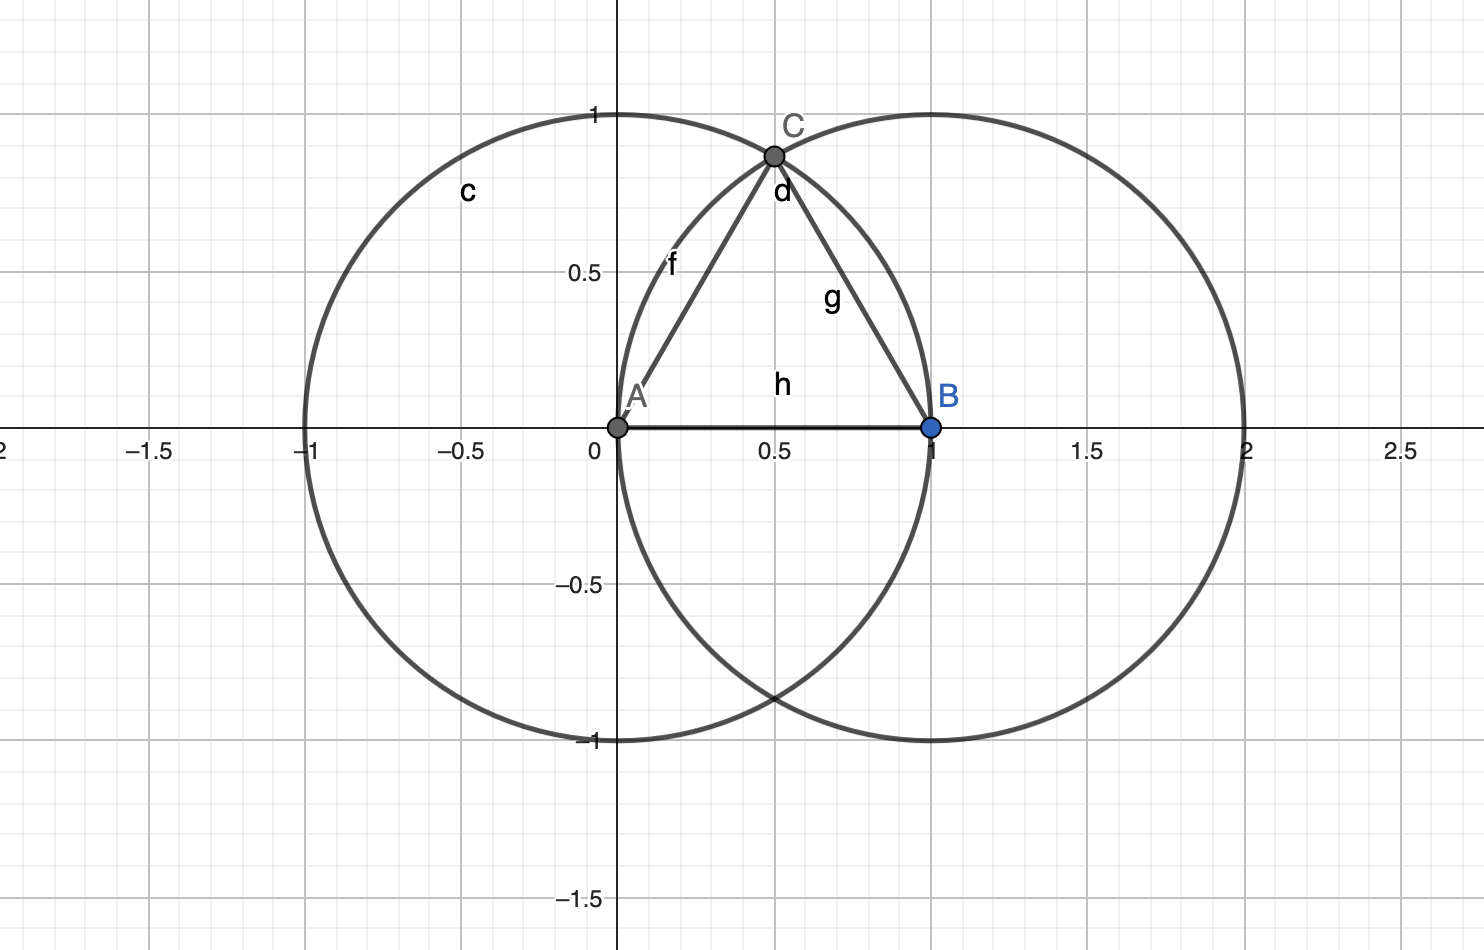
\includegraphics[width=0.5\textwidth]{triangle.png}
\end{center}
a field generated by 0, 1 is $\mathbb{Q}.$ with this equilateral trinalge we generated $\mathbb{Q}(\sqrt{3})$ \\ 
\subsection{intersecting lines }
\begin{align*}
    &\alpha_1 x + \beta_1 y = \gamma_1 \\
    &\alpha_2 x + \beta_2 y = \gamma_2 \\ 
    &\alpha_i, \beta_i, \gamma_i \in K \\ 
    &x, y \in K\\ 
\end{align*}
\subsection{intersecting line with circle }
\begin{align*}
    &\alpha x + \beta y = \gamma \\
    &(x- c_1)^2 + (y-c_2)^2 = r^2 \\ 
    &\text{quadratic in x}
\end{align*}
We may need to add square roots to the field. The degree of extension = 1 or 2. This is because the degree of the extension is the degree of the minimal polynomial. \\ 
Degree $[K : \mathbb{Q}]$ either stays the same or doubles. \\
$[K_{i+1}: \mathbb{Q}] = [K_{i+1} : K_i] \cdot [K_i : \mathbb{Q}]$ \\

\subsection{Intersecting two cricles }
\begin{align*}
    &(x-c_1)^2 + (y-c_2)^2 = r_1^2 \\
    &(x-d_1)^2 + (y-d_2)^2 = r_2^2 \\
    &c_i, d_i, r_i \in K_s
\end{align*}
Solving this system of equations will give us the intersection points. \\
\begin{align*}
    &x^2 - 2c_1x + c_1^2 + y^2 - 2c_2y + c_2^2 = r_1^2 \\
    &x^2 - 2d_1x + d_1^2 + y^2 - 2d_2y + d_2^2 = r_2^2 \\
    &(x-c_1)^2 + (y-c_2)^2 = r_1^2 \\
    &\text{linear equation x of y} \\ 
    &\rightarrow K_o = \mathbb{Q} \\ 
    &[K_s:\mathbb{Q}] = 2^j \quad j \in \mathbb{Z}, j \geq 0
\end{align*}
We must construct $\sqrt[3]{2}$ Using Eisenstein criteria $[\mathbb{Q}(\sqrt[3]{2}) : \mathbb{Q}] = 3$ This is not possible because: 

$$[K_s:\mathbb{Q}] ( = 2^j)= [K_s:\mathbb{Q}(\sqrt[3]{2})] \cdot [\mathbb{Q}(\sqrt[3]{2}):\mathbb{Q}] (=3)$$ 
\section{Trisecting an angle}

\end{document}
